\documentclass[12pt, titlepage]{article}

\usepackage{fullpage}
\usepackage[round]{natbib}
\usepackage{multirow}
\usepackage{booktabs}
\usepackage{tabularx}
\usepackage{graphicx}
\usepackage{float}
\usepackage{hyperref}
\hypersetup{
    colorlinks,
    citecolor=blue,
    filecolor=black,
    linkcolor=red,
    urlcolor=blue
}

%% Comments

\usepackage{color}

\newif\ifcomments\commentstrue %displays comments
%\newif\ifcomments\commentsfalse %so that comments do not display

\ifcomments
\newcommand{\authornote}[3]{\textcolor{#1}{[#3 ---#2]}}
\newcommand{\todo}[1]{\textcolor{red}{[TODO: #1]}}
\else
\newcommand{\authornote}[3]{}
\newcommand{\todo}[1]{}
\fi

\newcommand{\wss}[1]{\authornote{blue}{SS}{#1}} 
\newcommand{\plt}[1]{\authornote{magenta}{TPLT}{#1}} %For explanation of the template
\newcommand{\an}[1]{\authornote{cyan}{Author}{#1}}

%% Common Parts

\newcommand{\progname}{ProgName} % PUT YOUR PROGRAM NAME HERE
\newcommand{\authname}{Team \#, Team Name
\\ Student 1 name
\\ Student 2 name
\\ Student 3 name
\\ Student 4 name} % AUTHOR NAMES                  

\usepackage{hyperref}
    \hypersetup{colorlinks=true, linkcolor=blue, citecolor=blue, filecolor=blue,
                urlcolor=blue, unicode=false}
    \urlstyle{same}
                                


\newcounter{acnum}
\newcommand{\actheacnum}{AC\theacnum}
\newcommand{\acref}[1]{AC\ref{#1}}

\newcounter{ucnum}
\newcommand{\uctheucnum}{UC\theucnum}
\newcommand{\uref}[1]{UC\ref{#1}}

\newcounter{mnum}
\newcommand{\mthemnum}{M\themnum}
\newcommand{\mref}[1]{M\ref{#1}}

\begin{document}

\title{Module Guide for Hairesthetics}

\author{Team 18 \\ Charlotte Cheng
        \\ Marlon Liu
        \\ Senni Tan
        \\ Qiushi Xu
        \\ Hongwei Niu
        \\ Bill Song
}
\date{\today}

\maketitle

\pagenumbering{roman}

\section{Revision History}

\begin{tabularx}{\textwidth}{p{3cm}p{2cm}X}
\toprule {\bf Date} & {\bf Version} & {\bf Notes}\\
\midrule
Jan 16 & 0 & Rev0 MG\\
\bottomrule
\end{tabularx}

\newpage

\section{Reference Material}

This section records information for easy reference.

\subsection{Abbreviations and Acronyms}

\renewcommand{\arraystretch}{1.2}
\begin{tabular}{l l} 
  \toprule		
  \textbf{symbol} & \textbf{description}\\
  \midrule 
  AC & Anticipated Change\\
  DAG & Directed Acyclic Graph \\
  M & Module \\
  OS & Operating System \\
  R & Requirement\\
  SC & Scientific Computing \\
  \progname & Explanation of program name\\
  UC & Unlikely Change \\
  ML & Machine Learning \\
  UI & User Interface\\
  AI & Artificial Intelligence \\
  AR & Augumented Reality \\
  App & Application \\
  API & Application programming interface\\
  REST & Representational state transfer\\
  RGB & Red, Green, Blue \\
  macOS & Operating system developed by Apple Inc \\
  SRS & Software Requirement Specification \\
  VnVPlan & Validation and Verification Plan \\
  MG & Module Guide \\
  MIS & Module Interface Specification \\
  \bottomrule
\end{tabular}\\

\newpage

\tableofcontents

\listoftables

\listoffigures

\newpage

\pagenumbering{arabic}

\section{Introduction}

	\subsection{Overview}
	This project is to develop a software application that allows users to virtually simulate hairstyles and hair colors. The goal is to create a user-friendly, functional, and robust application that meets the essential functional requirements and non-functional requirements. The end result will be a software application that helps users easily and effectively experiment with different hairstyles and hair colors, providing an immersive and personalized virtual styling experience.
	
	\subsection{Context}
	This Module Guide(MG) of our project is developed after the Software Requirements Specification(SRS). The purpose of the MG is to explain the structure of modules based on selected design principles and patterns which further helps understand the project's functionalities based on the SRS. It also briefly introduces the services each module provides.
	
	\subsection{Design Principles}
	The design principles which would be used in the MG include information Hiding, high cohesion, low coupling, high fan-in, and low fan-out for module decomposition. Information Hiding includes identifying and encapsulating the expected changes. 

    \subsection{Design Pattern}
    Our project follows the MVC (model-view-controller) design pattern. MVC allows us to apply the separation of concern principle and breaks the complex problem into smaller sub-problems that can be solved in different modules. 

	\subsection{Document Structure}
\begin{itemize}

\item Anticipated and Unlikely Change

\item Module Hierarchy: It places modules related to the functional requirements in the behaviour hiding module.

\item Connection Between Requirements And Design: It provides the decisions of design that are needed to be made to realize the requirements 

\item Module Decomposition: It explains each module by following design principles.

\item Traceability Matrices: One matrix is between modules and requirements, the other is between modules and anticipated changes.

\item Uses Hierarchy: Diagram explains user hierarchy.

\item Project Schedule

\item Revision History
\end{itemize}	


\section{Anticipated and Unlikely Changes} \label{SecChange}

This section lists possible changes to the system. According to the likeliness
of the change, the possible changes are classified into two
categories. Anticipated changes are listed in Section \ref{SecAchange}, and
unlikely changes are listed in Section \ref{SecUchange}.

\subsection{Anticipated Changes} \label{SecAchange}

Anticipated changes are the source of the information that is to be hidden
inside the modules. Ideally, changing one of the anticipated changes will only
require changing the one module that hides the associated decision. The approach
adapted here is called design for
change.

\noindent \begin{itemize}

\item[AC\refstepcounter{acnum}\theacnum\label{LC_meaningfulLabel}:] 
This project will only result in the development of a MacOS app. However, an android application may also be developed to work with, or in place of, the MacOS application in the future.
\item[AC\refstepcounter{acnum}\theacnum\label{LC_meaningfulLabel}:] 
The application may be extended to offer compatibility as a web application.
\item[AC\refstepcounter{acnum}\theacnum\label{LC_meaningfulLabel}:] 
The application will not initially pursue functionality for users to "cut" their 3D simulated hair.
\item[AC\refstepcounter{acnum}\theacnum\label{LC_meaningfulLabel}:] 
\sout{The application may require more data for the facial recognition feature.}
\item[AC\refstepcounter{acnum}\theacnum\label{LC_meaningfulLabel}:] 
The load capacity of the system is initially set low for the first edition of this application. As demand for the application increases, the load capacity must also increase to support a larger user base.
\item[AC\refstepcounter{acnum}\theacnum\label{LC_meaningfulLabel}:] 
The application may be required to include new features as discovered through use of the system in real-world scenarios.
\item[AC\refstepcounter{acnum}\theacnum\label{LC_meaningfulLabel}:] 
The format of the
input and output data of facial recognition, hair modification, hair salon recommendation system.
\item[AC\refstepcounter{acnum}\theacnum\label{LC_meaningfulLabel}:] 
The interface style requirements might change since no metric has been provided for this by stakeholders. 
\item[AC\refstepcounter{acnum}\theacnum\label{LC_meaningfulLabel}:] 
The speed and latency requirements might change since no metric has been provided for this by stakeholders. 
\item[AC\refstepcounter{acnum}\theacnum\label{LC_meaningfulLabel}:] 
The precision and accuracy requirements might change since no metric has been provided for this by stakeholders. 


\end{itemize}

\subsection{Unlikely Changes} \label{SecUchange}

The module design should be as general as possible. However, a general system is
more complex. Sometimes this complexity is not necessary. Fixing some design
decisions at the system architecture stage can simplify the software design. If
these decisions should later need to be changed, then many parts of the design
will potentially need to be modified. Hence, it is not intended that these
decisions will be changed.

\noindent \begin{itemize}

\item[ULC\refstepcounter{ucnum}\theucnum\label{ULC_meaningfulLabel}:] 
Since several of the features might require exposing API endpoints, an offline-only version of the application is unlikely to be necessary. 
\item[ULC\refstepcounter{ucnum}\theucnum\label{ULC_meaningfulLabel}:] 
As the main demographic of this application is less computer literate, the ease of use of this application must remain a high priority consideration throughout the design of this system.
\item[ULC\refstepcounter{ucnum}\theucnum\label{ULC_meaningfulLabel}:] 
The application is designed to ensure that data will only be modified when necessary. 
\item[ULC\refstepcounter{ucnum}\theucnum\label{ULC_meaningfulLabel}:] 
The application is designed to ensure that only admins and supervisors will be able to unlock locked resources.
\item[ULC\refstepcounter{ucnum}\theucnum\label{ULC_meaningfulLabel}:] 
The application is designed to ensure that no inappropriate or offensive language towards any culture will be used.
\item[ULC\refstepcounter{ucnum}\theucnum\label{ULC_meaningfulLabel}:] 
The application is designed to ensure compliance with the Data Privacy Act of Canada. All user personal information will not be stored or used without consent. 
\item[ULC\refstepcounter{ucnum}\theucnum\label{ULC_meaningfulLabel}:] 
The application is designed to ensure that users are only able to see data that they have proper authorization for.
\item[ULC\refstepcounter{ucnum}\theucnum\label{ULC_meaningfulLabel}:] 
The application is designed to help users simulate hairstyles and hair colors virtually.
\item[ULC\refstepcounter{ucnum}\theucnum\label{ULC_meaningfulLabel}:] 
The primary user of this project is unlikely going to change since the project purpose is determined already, only certain types of users will be interested in this kind of application.
\item[ULC\refstepcounter{ucnum}\theucnum\label{ULC_meaningfulLabel}:] 
The client of this project is unlikely going to change because this project is a student capstone project and it has limited marketability.
\item[ULC\refstepcounter{ucnum}\theucnum\label{ULC_meaningfulLabel}:] 
The schedule and budget constraints are not likely going to change, because this project is a student capstone project. It needs to strictly follow SE4G06 course constraints.








\end{itemize}

\section{Module Hierarchy} \label{SecMH}

This section provides an overview of the module design. Modules are summarized
in a hierarchy decomposed by secrets in Table \ref{TblMH}. The modules listed
below, which are leaves in the hierarchy tree, are the modules that will
actually be implemented.

\begin{description}
\item [\refstepcounter{mnum} \mthemnum \label{mHH}:] Controller Module
\item [\refstepcounter{mnum} \mthemnum \label{mHH}:] Facial Recognition Module
\item [\refstepcounter{mnum} \mthemnum \label{mHH}:] Hair Color Module
\item [\refstepcounter{mnum} \mthemnum \label{mHH}:] Hair Style Module
\item [\refstepcounter{mnum} \mthemnum \label{mHH}:] Salon Recommendation Module
\item [\refstepcounter{mnum} \mthemnum \label{mHH}:] ML Model Module
\item [\refstepcounter{mnum} \mthemnum \label{mHH}:] Utility Module
\item [\refstepcounter{mnum} \mthemnum \label{mHH}:] Hair Color View Module
\item [\refstepcounter{mnum} \mthemnum \label{mHH}:] Hair Style View Module
\item [\refstepcounter{mnum} \mthemnum \label{mHH}:] Salon Recommendation View Module
\item [\refstepcounter{mnum} \mthemnum \label{mHH}:] Home View Module
\item [\refstepcounter{mnum} \mthemnum \label{mHH}:] Error View Module
\item [\refstepcounter{mnum} \mthemnum \label{mHH}:] Camera Module
\item [\refstepcounter{mnum} \mthemnum \label{mHH}:] Launch View Module
\end{description}

\begin{table}[H]
\centering
\begin{tabular}{p{0.3\textwidth} p{0.6\textwidth}}
\toprule
\textbf{Level 1} & \textbf{Level 2}\\
\midrule

{Hardware-Hiding Module} & M13 \\
\midrule

\multirow{7}{0.3\textwidth}{Behaviour-Hiding Module}
& M1\\
& M2\\
& M3\\
& M4\\
& M5\\
& M8\\
& M9\\
& M10\\
& M11\\
& M14\\
\midrule

\multirow{2}{0.3\textwidth}{Software Decision Module} & M6 \\  & M7\\
\bottomrule

\end{tabular}
\caption{Module Hierarchy}
\label{TblMH}
\end{table}

\section{Connection Between Requirements and Design} \label{SecConnection}

The design of the system is intended to satisfy the requirements developed in
the SRS. In this stage, the system is decomposed into modules. The connection
between requirements and modules is listed in Table~\ref{TblRT}.

\section{Module Decomposition} \label{SecMD}

Modules are decomposed according to the principle of ``information hiding''
proposed by David Parnas. The \emph{Secrets} field in a module
decomposition is a brief statement of the design decision hidden by the
module. The \emph{Services} field specifies \emph{what} the module will do
without documenting \emph{how} to do it. For each module, a suggestion for the
implementing software is given under the \emph{Implemented By} title. If the
entry is \emph{OS}, this means that the module is provided by the operating
system or by standard programming language libraries.  \emph{\progname{}} means the
module will be implemented by the \progname{} software.

The software architecture we use is the model-view-controller(MVC) architecture, it provides the principle of separation of concerns for our system as well as convenience for future addition and modification to certain components.
So we will follow the MVC architecture while decomposing our modules.


\subsection{Hardware Hiding Modules (M13)}

\begin{description}
\item[Secrets:]The implementation of the hardware adaptation.
\item[Services:]This module would allow the software to change and adapt the changes of hardware environment.
\item[Implemented By:] Swift
\end{description}

\subsubsection{Camera Module (M13)}

\begin{description}
\item[Secrets:]The implementation of access to camera.
\item[Services:]Provide access for the app to the device's camera.
\item[Implemented By:] Swift
\end{description}

\subsection{Behaviour-Hiding Module(M1, M2, M3, M4, M5, M8, M9, M10, M11, M12)}

\begin{description}
\item[Secrets:]The implementation of the behaviors of our application after processing user input
\item[Services:] The behavior-hiding modules includes both user-interface modules and backend logic modules. They serve as a communication layer between the
  hardware-hiding module and the software decision module.
\end{description}

\subsubsection{Controller Module (M1)}

\begin{description}
\item[Secrets:]Controllers to interact with the model and view components after processing the user input.
\item[Services:]Provides communication between the user inputs and modules and passes them to the UI.
\item[Implemented By:] Python / Swift
\item[Type of Module:] Abstract Data Type
\end{description}

\subsubsection{Facial Recognition Module (M2)}

\begin{description}
\item[Secrets:]Algorithm for detecting faces in the input image/video.
\item[Services:]Detect faces in the input image/video and provide facial landmarks
\item[Implemented By:] Python
\item[Type of Module:] Abstract Object
\end{description}

\subsubsection{Hair Color Module (M3)}

\begin{description}
\item[Secrets:]Algorithm for detecting the hair and changing its color on detected faces
\item[Services:] Perform hair re-coloring based on hair segmentation results.
\item[Implemented By:] Python
\item[Type of Module:] Abstract Object
\end{description}

\subsubsection{Hair Style Module (M4)}

\begin{description}
\item[Secrets:]Algorithm for adding new hair on detected faces
\item[Services:]Obtain position and rotation degree for adding AR hair model based on input user faces.
\item[Implemented By:] Python
\item[Type of Module:] Abstract Object
\end{description}

\subsubsection{Salon Recommendation Module (M5)}

\begin{description}
\item[Secrets:] The implementation of nearby salon recommendation.
\item[Services:] Highlight the nearby salons on the map according to the input address and provide a listing that can be filtered by rankings and distances.

\item[Implemented By:] Python, Google Map API
\item[Type of Module:] Abstract Object
\end{description}

\subsubsection{Hair Color View Module (M8)}

\begin{description}
\item[Secrets:] Algorithms and data structure for the hair color changing screen.
\item[Services:] Display the resulted color of hair when user changes the hair color.
\item[Implemented By:] Swift
\item[Type of Module:] Abstract Object
\end{description}

\subsubsection{Hair Style View Module (M9)}

\begin{description}
\item[Secrets:] Algorithms and data structure for hair style changing screen.
\item[Services:] Put the selected AR hair model to the detected face when user press the buttons accordingly.
\item[Implemented By:] Swift
\item[Type of Module:] Abstract Object
\end{description}

\subsubsection{Salon Recommendation View Module (M10)}

\begin{description}
\item[Secrets:] Algorithms and data structure for salon recommendation screen.
\item[Services:] Display nearby hair salon and display information about a chosen salon.
\item[Implemented By:] Python, Google Maps API
\item[Type of Module:] Abstract Object
\end{description}

\subsubsection{Home View Module (M11)}

\begin{description}
\item[Secrets:] Algorithms and data structure for displaying the home screen.
\item[Services:] Provide basic guidance and buttons for the users to start using the app.

\item[Implemented By:] Swift
\item[Type of Module:] Abstract Object
\end{description}

\subsubsection{Error View Module (M12)}

\begin{description}
\item[Secrets:] Algorithms and data structure for displaying the error screen.
\item[Services:] Provide details and guidance to errors happening in the application.
\item[Implemented By:] Swift
\item[Type of Module:] Abstract Object
\end{description}

\subsubsection{Launch View Module (M14)}

\begin{description}
\item[Secrets:] Algorithms and data structure for displaying the error screen.
\item[Services:] Provide details and status when loading the application.
\item[Implemented By:] Swift
\item[Type of Module:] Abstract Object
\end{description}

\subsection{Software Decision Module (M6, M7)}

\begin{description}
\item[Secrets:] The design decision based on mathematical models, and real-world objects in the form of data structures. It also includes libraries required to support behavioral functionalities.
\item[Services:] Includes data structure and algorithms used in the system that
  do not provide direct interaction with the user. 

\item[Implemented By:] Python
\end{description}

\subsubsection{ML Model Module (M6)}

\begin{description}
\item[Secrets:]Data structure for representing a pre-trained model
\item[Services:]  This module will provide functions to load the pre-trained model for hair segmentation if it's not already loaded. It also provides functions to interact with the model easily.
\item[Implemented By:] Python
\item[Type of Module:] Abstract Object
\end{description}

\subsubsection{Utility Module (M7)}

\begin{description}
\item[Secrets:]Utility functions for image processing
\item[Services:] This module will provide utility services and operations required for performing functional behaviors.
\item[Implemented By:] Python
\item[Type of Module:] Library
\end{description}

\section{Traceability Matrix} \label{SecTM}

This section shows two traceability matrices: between the modules and the
requirements and between the modules and the anticipated changes.

% the table should use mref, the requirements should be named, use something
% like fref
\begin{table}[H]
\centering
\begin{tabular}{p{0.2\textwidth} p{0.6\textwidth}}
\toprule
\textbf{Req.} & \textbf{Modules}\\
\midrule
FR1 & M8, M9\\
FR2 & M7\\
FR3 & M2, M6\\
FR6 & M2\\
FR7 & M2, M6\\
HM1 & M8\\
HM2 & M3\\
HM3 & M3\\
HM4 & M4, M6\\
HM5 & M9\\
HM7 & M7\\
HM8 & M4\\
HM9 & M8, M9\\
HM10 & M3, M6\\
HR1 & M10 \\
HR2 & M5 \\
HR3 & M10 \\
HR4 & M5 \\
\bottomrule
\end{tabular}
\caption{Trace Between Requirements and Modules}
\label{TblRT}
\end{table}

\begin{table}[H]
\centering
\begin{tabular}{p{0.2\textwidth} p{0.6\textwidth}}
\toprule
\textbf{AC} & \textbf{Modules}\\
\midrule
AC1 & M8, M9, M10, M11, M12\\
AC2 & Not applicable \\
AC3 & M4, M9 \\
AC4 & M6 \\
AC5 & Not applicable \\
AC6 & M1\\
AC7 & M2, M4, M5\\
AC8 & M8, M9, M10, M11, M12\\
AC9 & M5, M10\\
AC10 & M4, M9\\
\bottomrule
\end{tabular}
\caption{Trace Between Anticipated Changes and Modules}
\label{TblACT}
\end{table}

\section{Use Hierarchy Between Modules} \label{SecUse}

In this section, the uses hierarchy between modules is
provided. Two programs A and B that A {\em uses} B if
correct execution of B may be necessary for A to complete the task described in
its specification. That is, A {\em uses} B if there exist situations in which
the correct functioning of A depends upon the availability of a correct
implementation of B.  Figure \ref{FigUH} illustrates the use relation between
the modules. It can be seen that the graph is a directed acyclic graph
(DAG). Each level of the hierarchy offers a testable and usable subset of the
system, and modules in the higher level of the hierarchy are essentially simpler
because they use modules from the lower levels.

% \begin{figure}[H]
% \centering
% %\includegraphics[width=0.7\textwidth]{UsesHierarchy.png}

% \label{FigUH}
% \end{figure}

\subsection{Use Hierarchy Diagram}
\begin{center}
\begin{figure}[H]
% \graphicspath{ {component_diagram.jpg} }
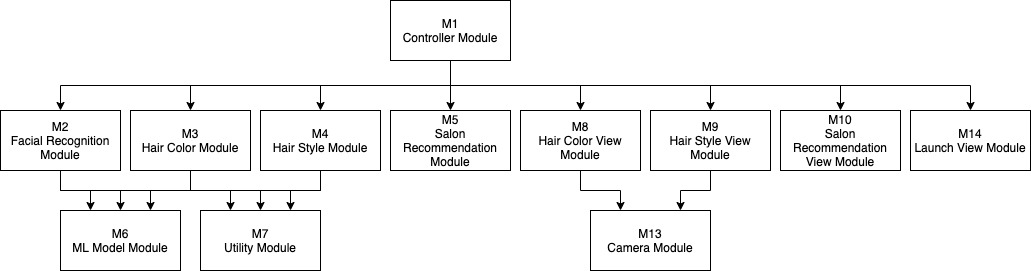
\includegraphics[width=1\textwidth]{Design/SoftArchitecture/use_hierarchy.jpg}
\caption{Use hierarchy among modules}
\label{FigUH} 
\end{figure}
\end{center}

\subsection{UML Diagram}
\begin{center}
\begin{figure}[]
% \graphicspath{ {component_diagram.jpg} }
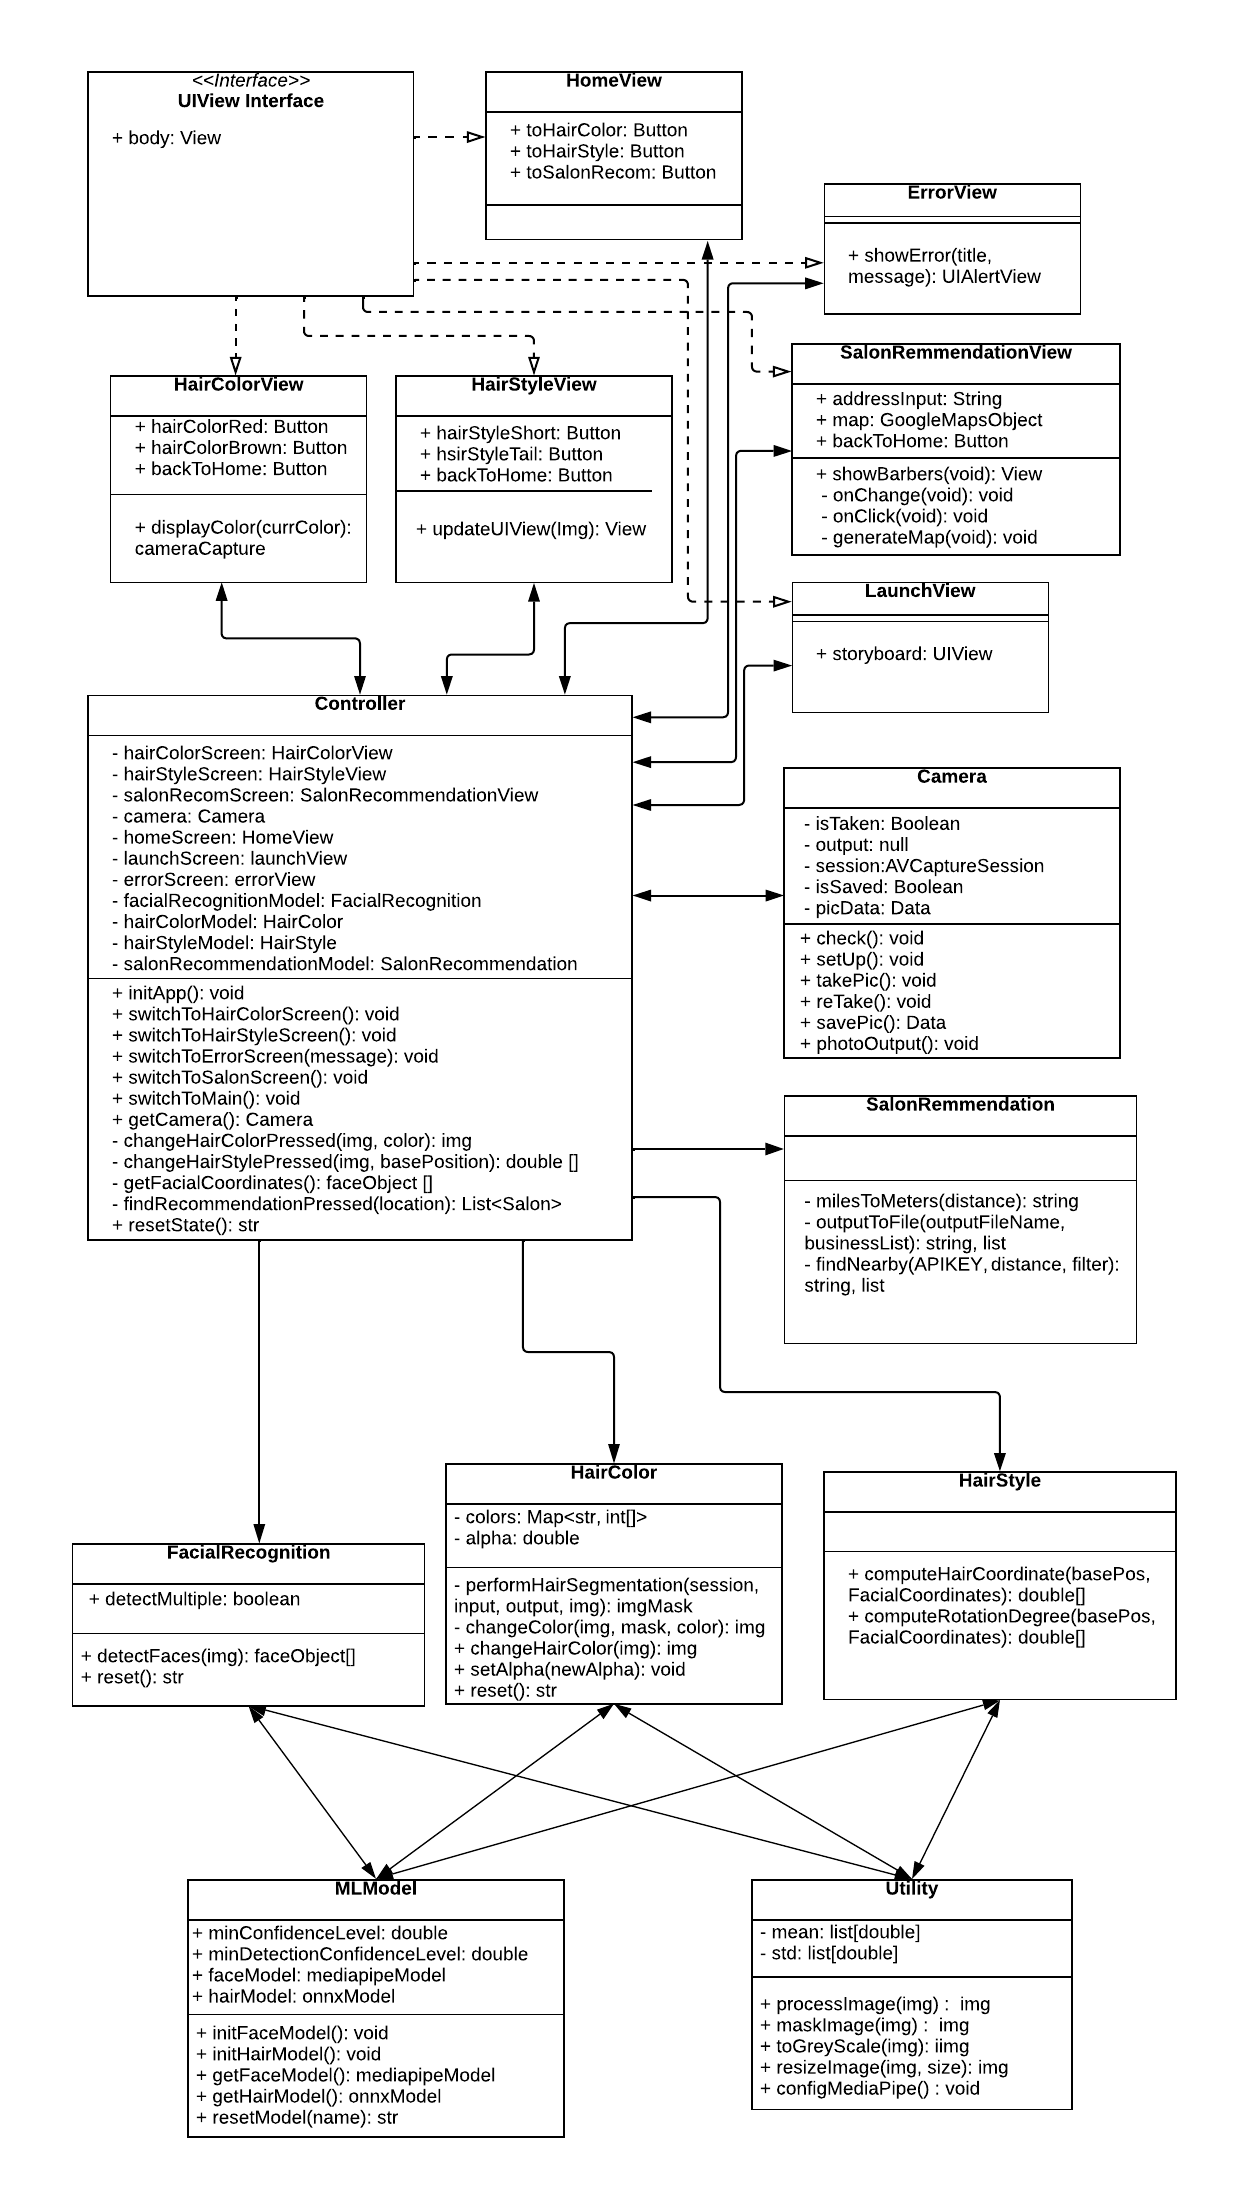
\includegraphics[width=0.8\textwidth, scale=0.8, keepaspectratio]{Design/SoftArchitecture/UML.png}
\caption{UML Diagram}
\label{FigUH} 
\end{figure}
\end{center}


%\section*{References}

% \bibliographystyle {plainnat}
% \bibliography{../../../refs/References}


\end{document}